\chapter{Appendix}





% \subsection{Google Image Bias}
% \subsection{More MoCo loss failure cases?}
% \begin{itemize}
%     \item long images 
% \end{itemize}



% \section{VOC2007 Linear Probe Accuracy}
% \begin{table}[t]
%     \centering
%     \begin{tabular}{lc}
%     \toprule
%         Model & VOC2007 \\
%     \midrule
%     \textit{Fixed dataset Self-Supervised} \\
%         \;\;\; MoCo-v3~\cite{chen2021empirical} (VOC2007 pre-train)   & 58.0 \\
%     \midrule
%     \textit{No label set information} \\
%         \;\;\;Random exploration                                      &  64.8 \\ % expID 1138
%         \;\;\;Ours                                                    & 63.4 \\ % expID 1139
%         \;\;\;Ours++                                                  & 64.9 \\ % expID 1142
%     \midrule 
%     \textit{Use label set information} \\       
%         \;\;\;Search labels only                                      & 60.8 \\ % expID 1141
%         \;\;\;Labels + semantically relevant terms                    & 65.3 \\ % expID 1136
%         \;\;\;Ours                                                    & 65.4 \\ % expID 1140
%         \;\;\;Ours++                                                  & \textbf{72.9} \\ % expID 1143
%     \bottomrule
%     \end{tabular}
%     \caption{\textbf{Linear probe accuracy on VOC2007}. 
%     }
%     \label{tab:voc2007}
% \end{table}

% VOC categories are broad, unlike the fine-grained classes in Birdsnap, Flowers, Food, and Pets. Thus, comparing against ImageNet pre-training or CLIP would be unfair since these datasets are diverse, cleaned, class-balanced, and entirely relevant to VOC. Thus, we start from and compare against a MoCo-v3 checkpoint that has only been pre-trained on VOC2007. We report the linear probe accuracy for Pascal VOC2007 in \cref{tab:voc2007}. We find that Internet Explorer improves faster than randomly searching the Internet, especially when it has label set information to help guide it. 

% \section{More seeds}



\section{Progression of downloaded images}
\label{sec:progression_downloaded_imgs}
Just as Fig. 4 in the main paper showed how Internet Explorer progressively discovers useful data when targeting the Pets dataset, \cref{fig:birdsnap_progression}, \cref{fig:flowers_progression}, \cref{fig:food_progression}, and \cref{fig:voc_progression} show the progression of downloaded images when targeting Birdsnap, Flowers, Food, and VOC respectively. Note that this analysis is in the self-supervised setting, without any knowledge of the label set. 

\begin{figure*}
    \centering
    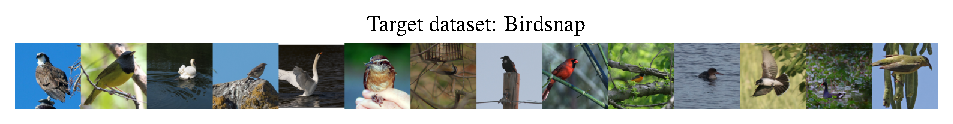
\includegraphics{figures/birdsnap_targets.pdf} \\
    \vspace{-0.8em}
    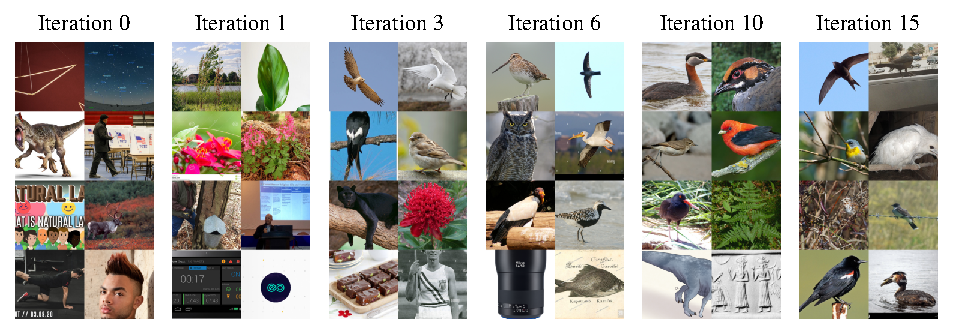
\includegraphics{figures/birdsnap-progression-1146-2col.pdf}
    \caption{\textbf{Progression of downloaded Birdsnap images.} This corresponds to Ours++ without using label set information. }
    \label{fig:birdsnap_progression}
\end{figure*}

\begin{figure*}
    \centering
    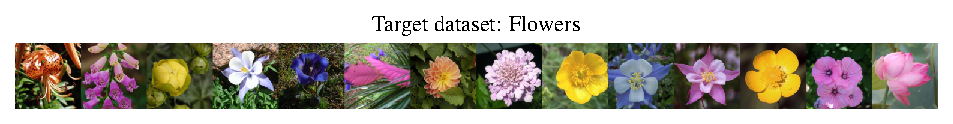
\includegraphics{figures/flowers_targets.pdf} \\
    \vspace{-0.8em}
    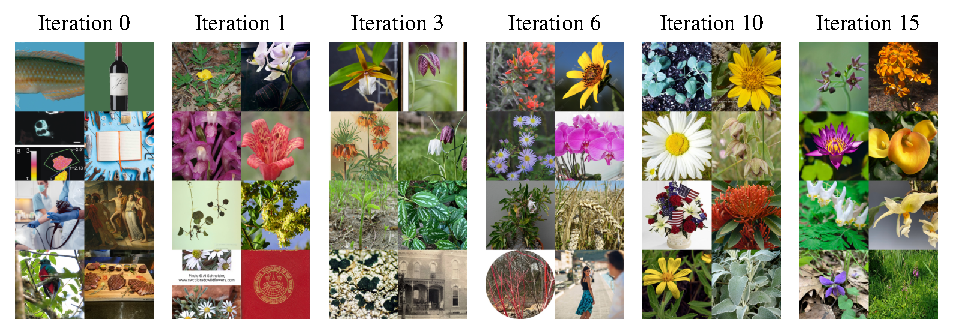
\includegraphics{figures/flowers-progression-1150-2col.pdf}
    \caption{\textbf{Progression of downloaded Flowers images.} This corresponds to Ours++ without using label set information. }
    \label{fig:flowers_progression}
\end{figure*}

\begin{figure*}
    \centering
    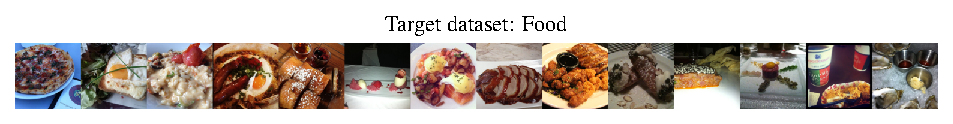
\includegraphics{figures/food_targets.pdf} \\
    \vspace{-0.8em}
    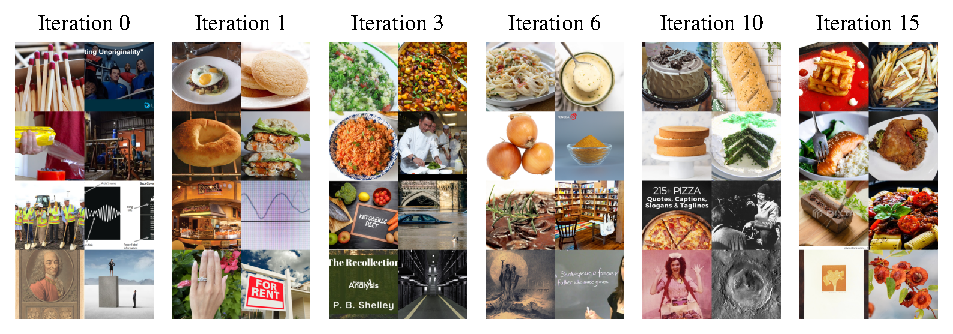
\includegraphics{figures/food-progression-1148-2col.pdf}
    \caption{\textbf{Progression of downloaded Food images.} This corresponds to Ours++ without using label set information. }
    \label{fig:food_progression}
\end{figure*}

\begin{figure*}
    \centering
    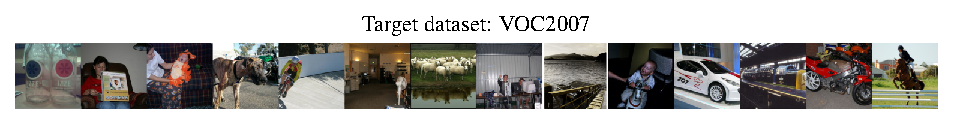
\includegraphics{figures/voc_targets.pdf} \\
    \vspace{-0.8em}
    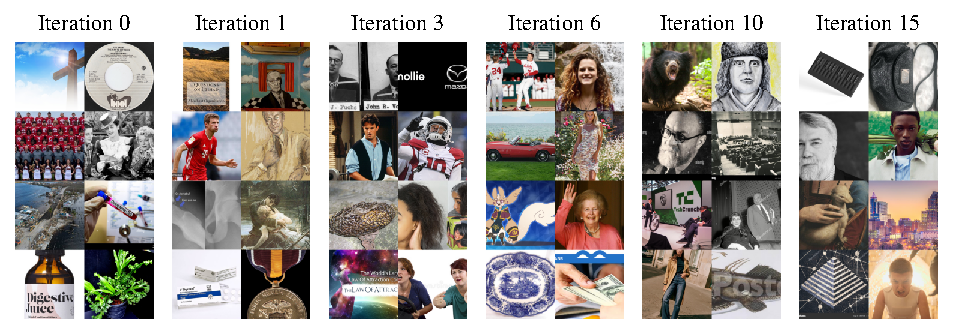
\includegraphics{figures/voc-progression-1156-2col.pdf}
    \caption{\textbf{Progression of downloaded VOC2007 images.} This corresponds to Ours++ without using label set information. }
    \label{fig:voc_progression}
\end{figure*}

% \section{Other experiments:}
% \begin{itemize}
% \item do we need GP or not 
% \item do we need std + mean or not 
% \end{itemize}

%%%%%%%%%%%%%%%%%%%%%%%%%%%%%%%%%%%%%%%%%%%%%%%%%%%%%%%%%%%%%%%%%%%%%%%%%%%%%%%
%%%%%%%%%%%%%%%%%%%%%%%%%%%%%%%%%%%%%%%%%%%%%%%%%%%%%%%%%%%%%%%%%%%%%%%%%%%%%%%

\section{Additional Figures}
\begin{figure}
    \centering
    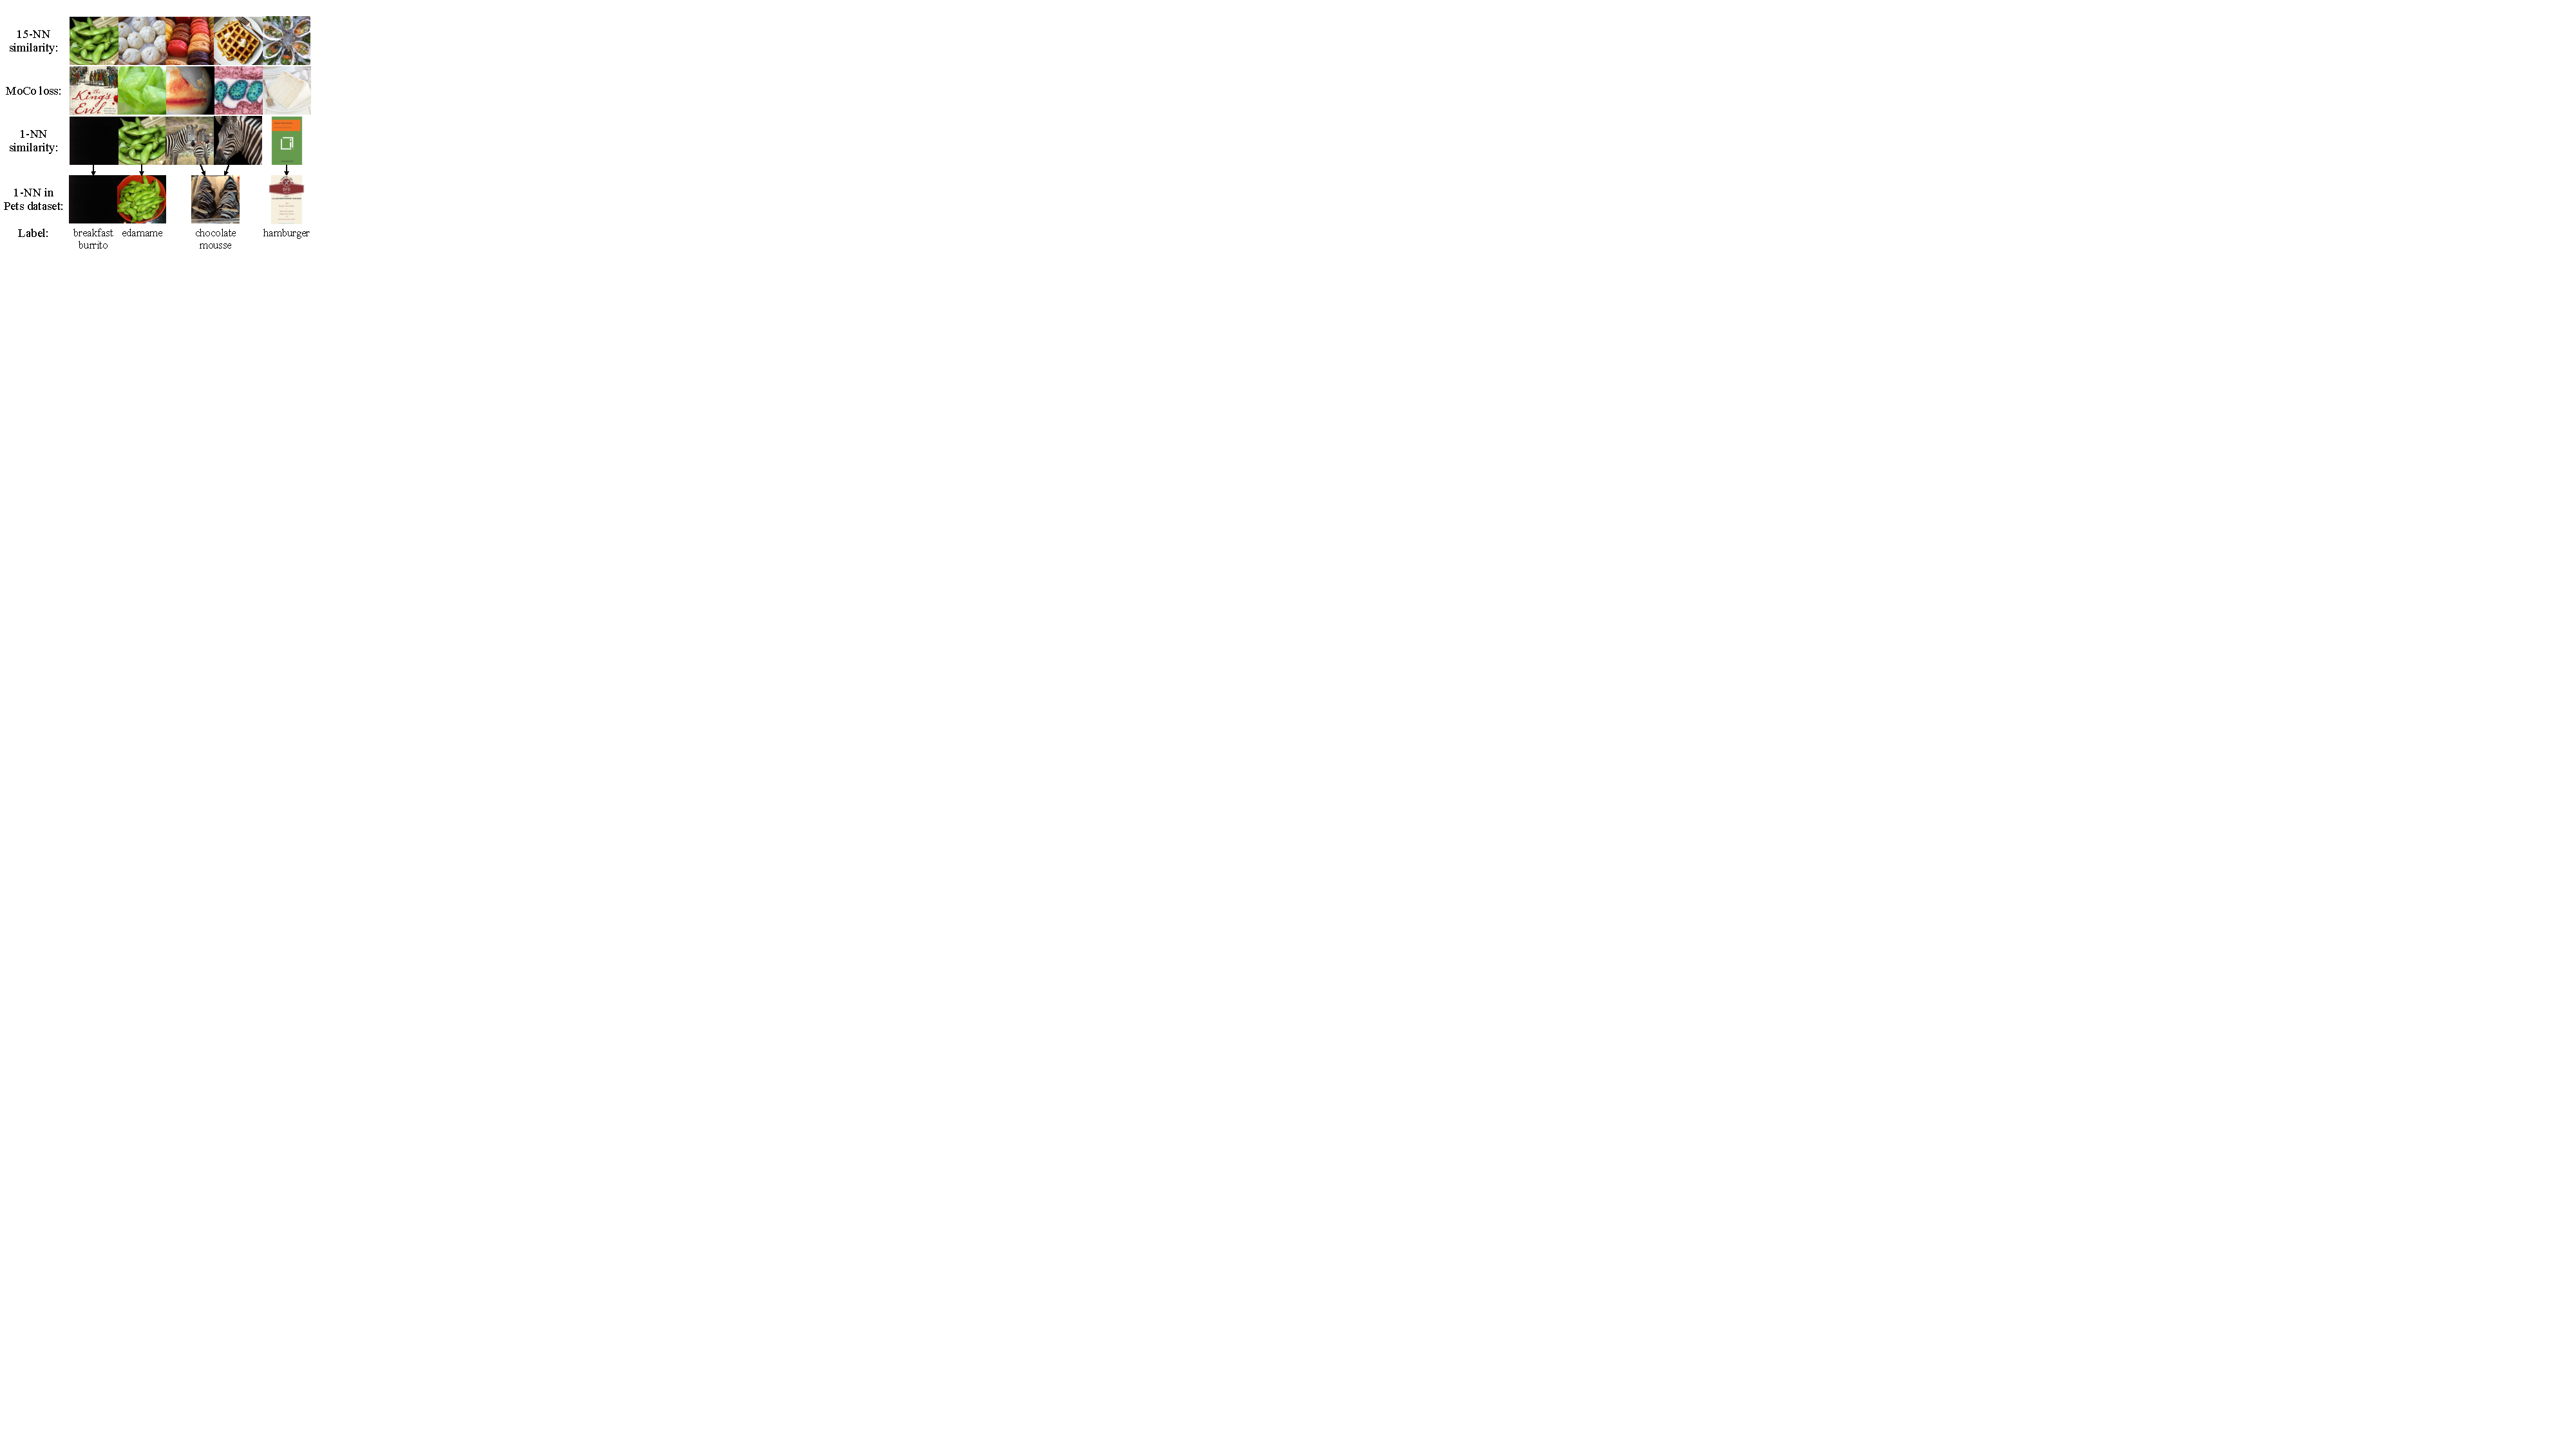
\includegraphics[width=0.5\linewidth]{figures/reward_ranking.pdf}
    % \vspace{-0.25in}
    \caption{\textbf{Top images preferred by different rewards.} We show the top 5 downloaded images ranked by 3 possible image rewards on the Food dataset. 15-NN (ours) prefers a variety of food images, whereas MoCo prefers noisy images out of the training distribution. 1-NN is thrown off by outliers in the Food dataset and thus prefers black images, text, and zebras.}
    \label{fig:reward_ranking}
    % \vspace{-0.06in}
\end{figure}

%%% Local Variables:
%%% coding: utf-8
%%% mode: latex
%%% TeX-engine: xetex
%%% TeX-master: "../thesis"
%%% End: